\documentclass[11pt]{article}

\usepackage[a4paper]{geometry}
\geometry{left=2.0cm,right=2.0cm,top=3cm,bottom=2.5cm}
\usepackage{setspace}
\setstretch{1.5}
\usepackage{ctex}
\usepackage{amsmath,amsfonts,graphicx,amssymb,bm,amsthm}
\usepackage{algorithm,algorithmicx}
\usepackage[noend]{algpseudocode}
\usepackage{fancyhdr}
\usepackage{booktabs}
\usepackage{array}
\usepackage{listings}
\usepackage{listingsutf8}
\usepackage{xcolor}

% 代码高亮设置，保持与HW2一致
\lstset{
	language=Python,
	basicstyle=\ttfamily\small,
	numbers=left,
	numberstyle=\tiny\color{teal!70!black},
	showstringspaces=false,
	breaklines=true,
	frame=single,
	rulecolor=\color{black},
	framerule=0.6pt,
	framesep=4pt,
	xleftmargin=6pt,
	backgroundcolor=\color{gray!4},
	inputencoding=utf8,
	columns=fullflexible,
	keywordstyle=\bfseries\color{blue!70!black},
	commentstyle=\itshape\color{green!50!black},
	stringstyle=\color{red!60!black},
	identifierstyle=\color{violet!70!black},
	emphstyle=\bfseries\color{orange!80!black},
	tabsize=4
}
\newcolumntype{M}[1]{>{\centering\arraybackslash}m{#1}}
\renewcommand{\lstlistingname}{代码片段}
\renewcommand{\lstlistlistingname}{代码列表}

\begin{document}
	\pagestyle{fancy}
	\lhead{\kaishu 中国科学院大学}
	\chead{}
	\rhead{\kaishu 2025年秋季学期\qquad 人工智能原理：模型与算法}
	
	\begin{center}
		{\LARGE \bf 课程作业4：基于PPO算法的倒立摆控制} 
	\end{center}
	\begin{center}
		\large\kaishu{尧祥临 202518023406038 前沿交叉科学学院}
	\end{center}

	\section{任务介绍}
	本次作业的目标是实现近端策略优化（Proximal Policy Optimization, PPO）算法，并使用该算法在OpenAI Gym的 \texttt{CartPole-v1} 环境中训练智能体，实现对倒立摆的有效控制，目标是使智能体在尽可能多的时间步（500步）内保持倒立摆的平衡。

	\section{模型架构}
    PPO算法是一种基于策略梯度的强化学习方法，针对TRPO算法存在的重要性比例带来的大方差以及求解约束优化问题的困难等不足，在其基础上进行简化和改进，保留了策略稳定性。与课程ppt中介绍的PPO算法一致，这里采用了Clip截断式优化目标、GAE广义优势估计和自适应KL惩罚的方法来提升训练的稳定性和效率。
    
    \subsection{Actor-Critic框架}
    与使用蒙特卡洛采样直接估计回报的策略梯度方法不同，PPO算法采用了Actor-Critic框架。其中Actor网络负责输出动作的概率分布，Critic网络则负责估计状态值函数；在训练过程中，Critic要学会准确估计当前演员策略的动作价值，而Actor则通过Critic提供的价值估计来更新策略，从而实现策略的改进。

    具体而言，Actor网络用于估计在给定状态 $s$ 下采取动作 $a$ 的概率分布 $\pi_\theta(a|s)$，其目标是最大化期望回报。
        \begin{equation}
            \pi_\theta(a|s) \approx P(A_t=a | S_t=s)
        \end{equation}
    而对于Critic网络，在PPO中通常估计\textbf{状态价值函数} $V_\Phi(s)$，利用 $V_\Phi(s)$ 可以构建优势函数 $A(s,a)$ 来指导 Actor 更新：
        \begin{equation}
            V_\Phi(s) \approx \mathbb{E}[R_t + \gamma V(S_{t+1}) | S_t=s]
        \end{equation}

    
    \subsection{算法核心优化}
    \subsubsection{Clip截断式优化目标}
    为了避免策略更新步长过大导致性能急剧下降，PPO引入了Clip机制。首先定义概率比率$r_t(\theta)$：
    \begin{equation}
        r_t(\theta) = \frac{\pi_\theta(a_t|s_t)}{\pi_{\theta_{\text{old}}}(a_t|s_t)}
    \end{equation}
    其中$\pi_\theta$是新策略，$\pi_{\theta_{\text{old}}}$是旧策略。
    
    截断目标函数 $L^{CLIP}(\theta)$ 如下所示，旨在为Conservative Policy Iteration（CPI）构建下界：
    \begin{equation} 
        L^{CLIP}(\theta) = \hat{\mathbb{E}}_t \left[ \min(r_t(\theta)\hat{A}_t, \text{clip}(r_t(\theta), 1-\varepsilon, 1+\varepsilon)\hat{A}_t) \right]
    \end{equation}
    其中 $\hat{A}_t$ 是优势函数的估计值，$\varepsilon$ 是一个超参数，通常设置为0.2，用于限制 $r_t(\theta)$ 在 $[1-\varepsilon, 1+\varepsilon]$ 区间内。
    \begin{itemize}
        \item 当 $\hat{A}_t > 0$ 时，目标是增大 $r_t(\theta)$，但截断机制限制其最大不超过 $1+\varepsilon$。
        \item 当 $\hat{A}_t < 0$ 时，目标是减小 $r_t(\theta)$，但截断机制限制其最小不低于 $1-\varepsilon$。
    \end{itemize}
    这种机制确保了策略更新不会偏离旧策略太远，从而保证了训练的稳定性。
    \subsubsection{GAE广义优势估计}
    广义优势估计（Generalized Advantage Estimation, GAE）用于计算优势函数 $\hat{A}_t$，定义为多步时间差分误差的加权和：
    \begin{equation}
        \hat{A}_t = \sum_{k=0}^{\infty} (\gamma\lambda)^k \delta_{t+k}
    \end{equation}
    其中 $\delta_t = r_t + \gamma V(s_{t+1}) - V(s_t)$ 是单步时间差分误差。参数 $\lambda \in [0,1]$ 控制方差与偏差的权衡。

    \subsubsection{自适应KL惩罚}
    除了截断约束外，PPO还可以通过在目标函数中加入KL散度惩罚项来限制策略更新幅度。带KL惩罚的目标函数为：
    \begin{equation}
        L^{KLPEN}(\theta) = \hat{\mathbb{E}}_t \left[ r_t(\theta)\hat{A}_t - \beta \text{KL}[\pi_{\theta_{\text{old}}}(\cdot|s_t) | \pi_\theta(\cdot|s_t)] \right]
    \end{equation}
    其中 $\beta$ 是自适应调整的惩罚系数。在每次更新后，根据计算出的KL散度平均值 $d$ 动态调整 $\beta$：
    \begin{itemize}
        \item 如果 $d < d_{\text{targ}} / 1.5$，说明更新幅度过小，减小惩罚：$\beta \leftarrow \beta / 2$
        \item 如果 $d > d_{\text{targ}} \times 1.5$，说明更新幅度过大，增大惩罚：$\beta \leftarrow \beta \times 2$
    \end{itemize}

    \section{实现细节}
    \subsection{工具函数实现}
    \texttt{compute\_advantage}函数用于计算GAE优势函数，在接收TD误差 $\delta_t$ 序列，通过逆序递归方式计算优势函数 $\hat{A}_t$。
    \begin{lstlisting}
def compute_advantage(gamma, lmbda, td_delta):
    td_delta = td_delta.detach().numpy()
    advantage_list = []
    advantage = 0.0
    for delta in td_delta[::-1]:    # 逆序遍历计算GAE
        advantage = gamma * lmbda * advantage + delta
        advantage_list.append(advantage)
    advantage_list.reverse()    # 计算完成后翻转回正序
    return torch.tensor(np.array(advantage_list), dtype=torch.float)
    \end{lstlisting}

    \texttt{train\_on\_policy\_agent} 函数则实现了PPO训练循环，在一个Episode中收集完整的轨迹数据（包括State, Action, Reward等），然后用于更新策略的训练。

    \begin{lstlisting}
def train_on_policy_agent(env, agent, num_episodes):
    # ......
    for i_episode in range(num_episodes):
        transition_dict = {'states': [], 'actions': [], 'next_states': [], 'rewards': [], 'dones': []}
        state, info = env.reset()
        done = False
        while not done:
            action = agent.take_action(state)
            next_state, reward, terminated, truncated, _ = env.step(action)
            done = terminated or truncated
            transition_dict['states'].append(state)
            transition_dict['actions'].append(action)
            transition_dict['next_states'].append(next_state)
            transition_dict['rewards'].append(reward)
            transition_dict['dones'].append(done)
            state = next_state
        agent.update(transition_dict)
    # ......
    \end{lstlisting}

    \subsection{Actor-Critic网络设计}
    这里我构建了两个MLP神经网络分别作为Actor和Critic。PolicyNet，也就是Actor以状态维度的向量作为输入，经过一个包含128维的隐藏层并以ReLU为激活函数，最后通过Softmax层输出概率分布。ValueNet，也就是Critic采用类似的结构，但输出层为一个线性单元，用于输出状态价值的估计。
    \begin{lstlisting}
class PolicyNet(torch.nn.Module):
    def __init__(self, state_dim, hidden_dim, action_dim):
        super(PolicyNet, self).__init__()
        self.fc1 = torch.nn.Linear(state_dim, hidden_dim)
        self.fc2 = torch.nn.Linear(hidden_dim, action_dim)

    def forward(self, x):
        x = F.relu(self.fc1(x))
        return F.softmax(self.fc2(x), dim=1)

class ValueNet(torch.nn.Module):
    def __init__(self, state_dim, hidden_dim):
        super(ValueNet, self).__init__()
        self.fc1 = torch.nn.Linear(state_dim, hidden_dim)
        self.fc2 = torch.nn.Linear(hidden_dim, 1)

    def forward(self, x):
        x = F.relu(self.fc1(x))
        return self.fc2(x)
    \end{lstlisting}

    \subsection{策略更新逻辑}
    在策略更新阶段，计算Actor的损失时，这里采用了Clip截断机制与自适应KL惩罚相结合的策略：一方面通过\lstinline|torch.clamp|来限制概率比率的变化范围，另一方面计算新旧策略的KL散度作为惩罚项加入总损失中。此外，在每次更新结束后，还会根据KL散度的实际值动态调整惩罚系数$\beta$：
    \begin{lstlisting}
def update(self, transition_dict):
    # ......
    td_target = rewards + self.gamma * self.critic(next_states) * (1 - dones)   # 计算时间差分目标
    td_delta = td_target - self.critic(states)  # 计算时间差分误差
    advantage = utils.compute_advantage(self.gamma, self.lmbda, td_delta.cpu()).to(self.device)
    advantage = (advantage - advantage.mean()) / (advantage.std() + 1e-8)   # 优势归一化
    old_log_probs = torch.log(self.actor(states).gather(1, actions)).detach()  # 旧策略的log概率
    for _ in range(self.epochs):
        log_probs = torch.log(self.actor(states).gather(1, actions))    # 新策略的log概率
        ratio = torch.exp(log_probs - old_log_probs)
        surr1 = ratio * advantage
        surr2 = torch.clamp(ratio, 1 - self.eps, 1 + self.eps) * advantage  # Clip部分
        clip_loss = -torch.min(surr1, surr2)
        kl_div = torch.mean(old_log_probs - log_probs)
        kl_loss = self.kl_beta * kl_div # KL惩罚项
        actor_loss = torch.mean(clip_loss + kl_loss)
        critic_loss = torch.mean(F.mse_loss(self.critic(states), td_target.detach()))  
        self.actor_optimizer.zero_grad()
        self.critic_optimizer.zero_grad()
        actor_loss.backward()
        critic_loss.backward()
    # ......
    with torch.no_grad():
        kl_d = torch.mean(old_log_probs - new_log_probs).item() # 计算所有epoch训练完成之后最新的KL散度
    if kl_d < self.kl_target / 1.5:
        self.kl_beta /= 2
    elif kl_d > self.kl_target * 1.5:
        self.kl_beta *= 2
    \end{lstlisting}

    \subsection{超参数设置}
    训练中具体的超参数设置如下表所示，另外优化器选择了AdamW优化器.
    \begin{table}[htbp]
        \centering
        \caption{PPO 算法超参数设置}
        \begin{tabular}{ccc}
            \toprule
            参数名称 & 变量名 & 设定值 \\
            \midrule
            Actor Learning Rate & \lstinline|actor_lr| & 1e-3 \\
            Critic Learning Rate & \lstinline|critic_lr| & 1e-2 \\
            Hidden Layer Size & \lstinline|hidden_dim| & 128 \\
            Discount Factor & \lstinline|gamma| & 0.98 \\
            GAE Parameter & \lstinline|lmbda| & 0.95 \\
            Clip Epsilon & \lstinline|eps| & 0.2 \\
            KL Target & \lstinline|kl_target| & 0.01 \\
            Initial KL Beta & \lstinline|kl_beta| & 0.5 \\
            Number of Episodes & \lstinline|num_episodes| & 500 \\
            Update Epochs & \lstinline|epochs| & 10 \\
            \bottomrule
        \end{tabular}
    \end{table}

	\section{实验结果与分析}
    \subsection{训练过程分析}
    如图\ref{fig:rewards}所示，经过500个episode的训练，平均returns逐渐提升，并最终稳定在接近500的水平，可以认为模型已经学会了保持倒立摆的平衡。可以看到实际上在约150个episode的时候模型的平均returns已经有了显著的提升并接近500，但是此后的训练过程中出现了较大的波动。该图已经经过平滑处理，在原始曲线图像中波动幅度更大，虽然整体趋势保持了一致，但这仍然反映出强化学习训练过程中的不稳定性。
    \begin{figure}[htbp]
        \centering
        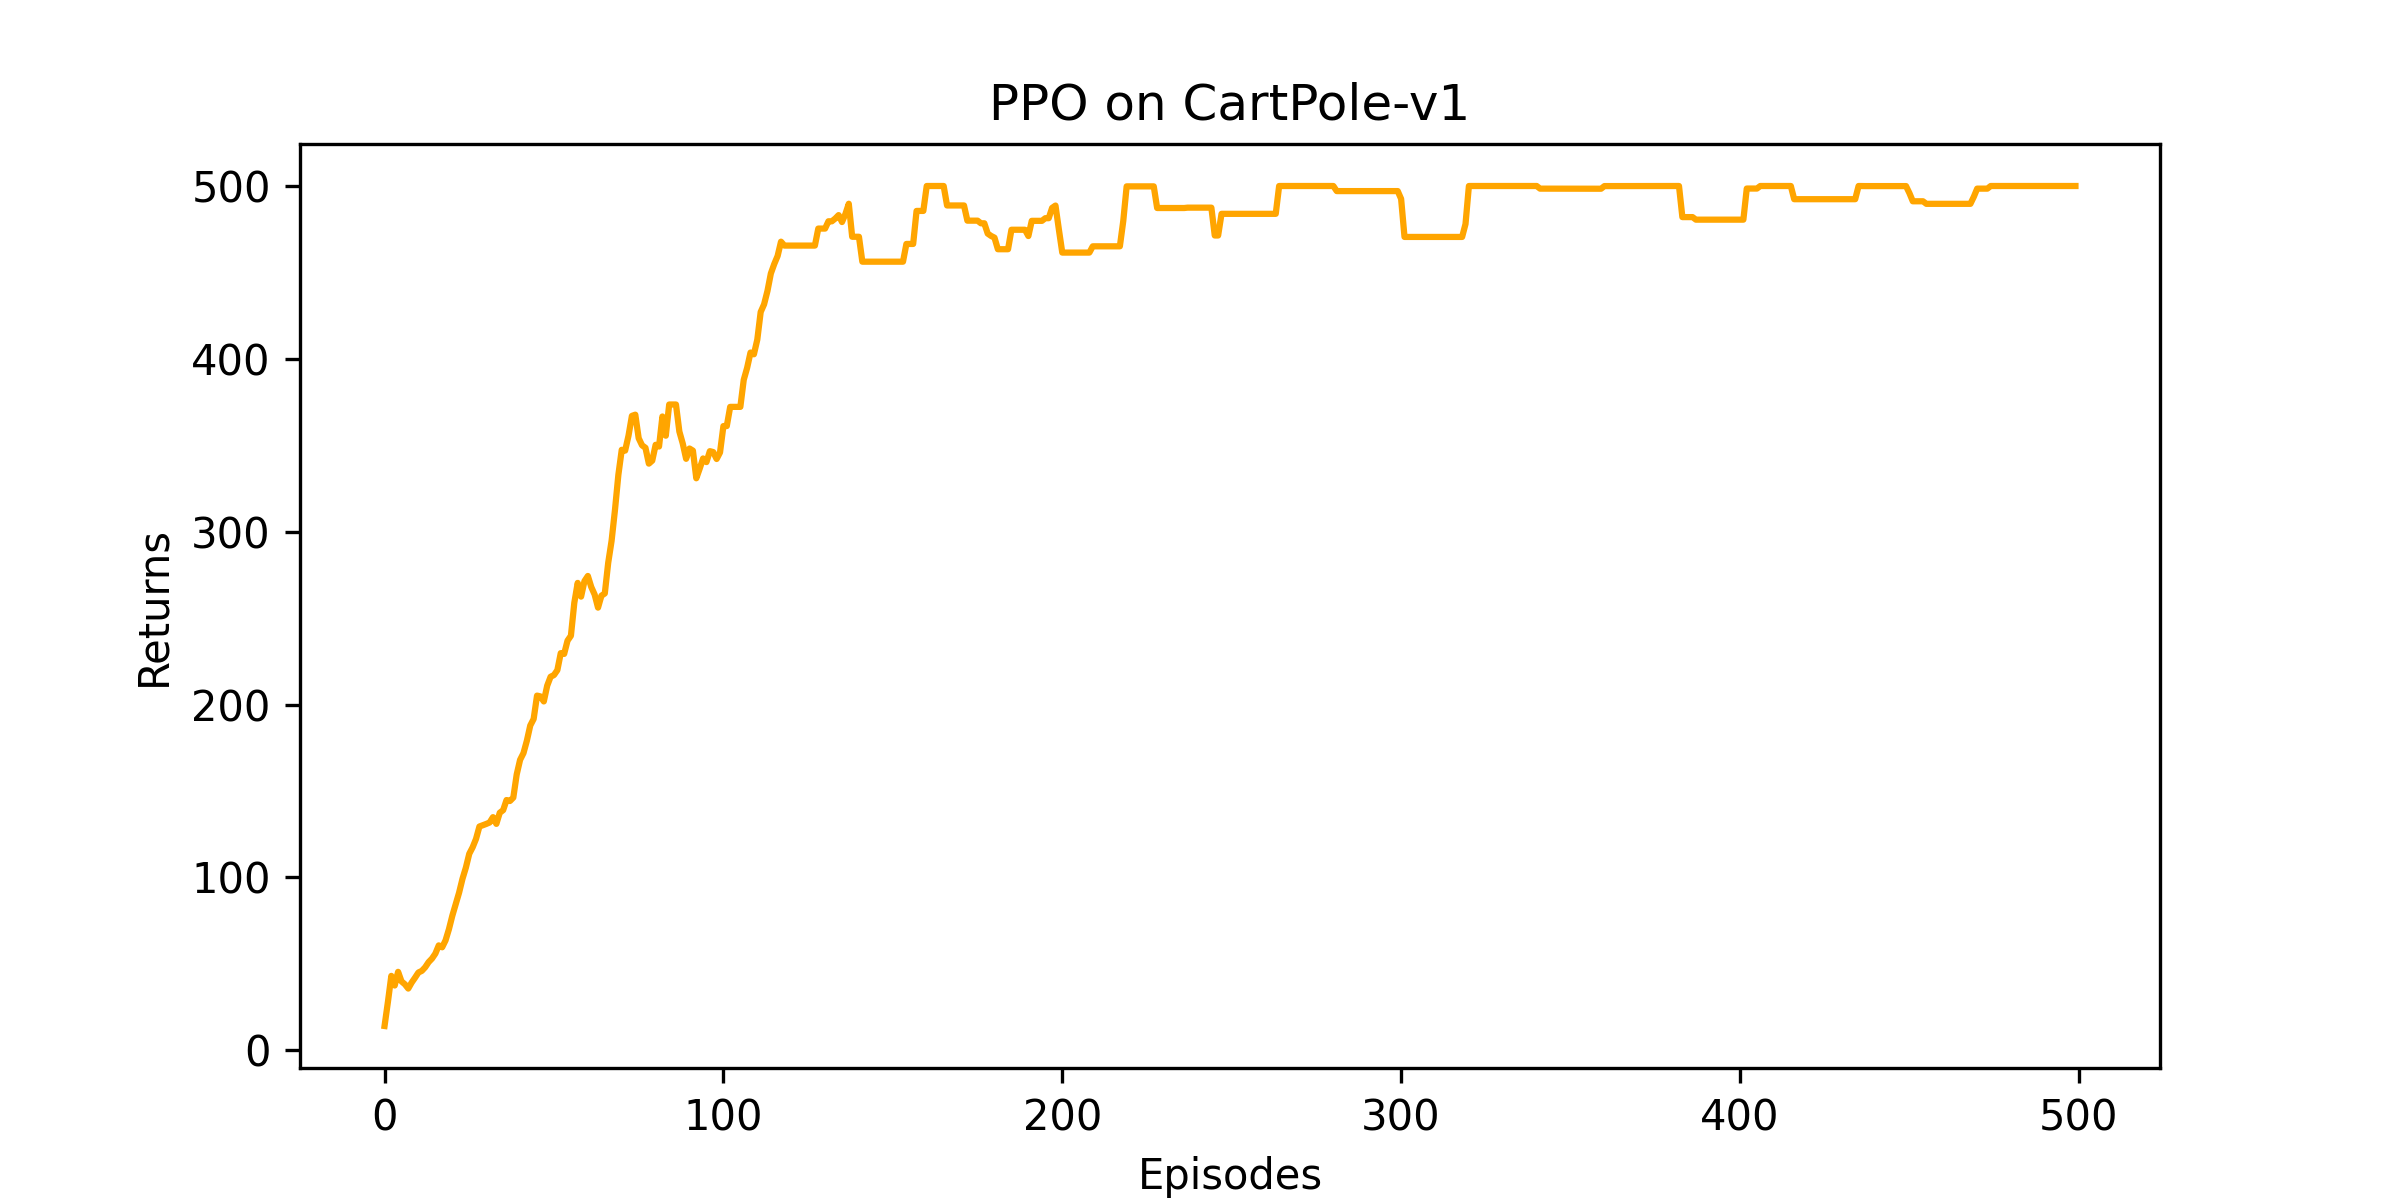
\includegraphics[width=0.8\textwidth]{../Figure/ppo_cartpole_returns_smooth.png} 
        \caption{训练过程中returns的变化趋势}
        \label{fig:rewards}
    \end{figure}

    图\ref{fig:actor_losses}和图\ref{fig:critic_losses}分别展示了训练过程中Actor和Critic的损失值变化情况。可以看到，随着训练的进行，Actor损失值由于其定义，是从负值开始逐渐趋近于零，虽然其波动非常大，但是仍然能看出相比训练初期有所改善，更加趋近于0。另一边，Critic损失值则没有表现出明显的趋势，除部分episode出现较大的波动外，整体维持在一个相对较小的正值，这与每一回合的奖励和状态转移都带有随机性有关，因此Critic损失值补收敛到0是合理的。
    \begin{figure}[htbp]
        \centering
        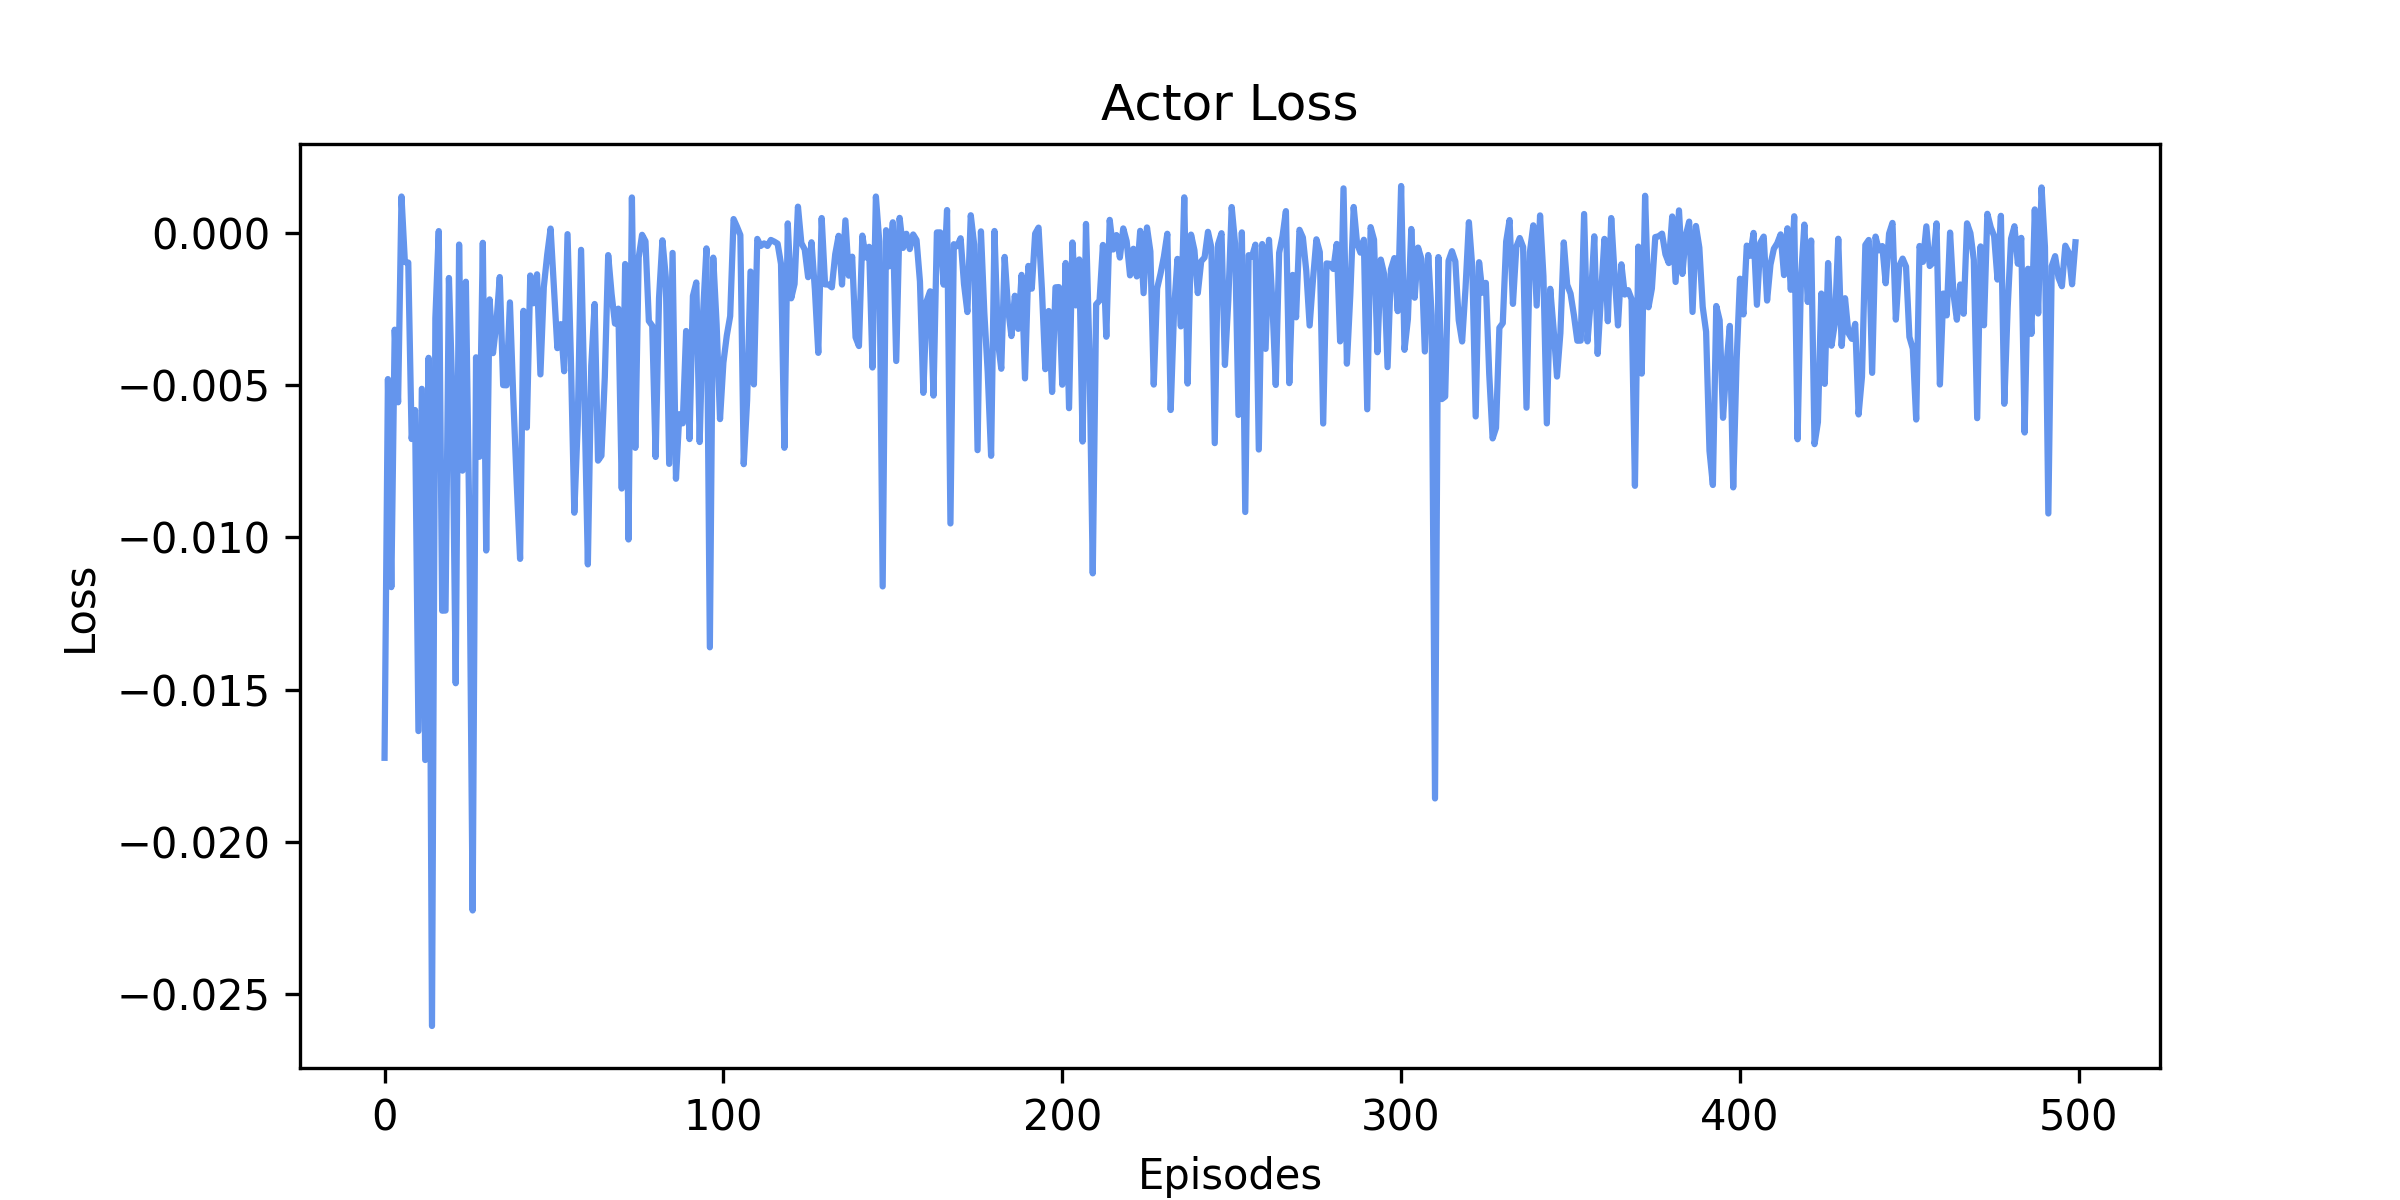
\includegraphics[width=0.8\textwidth]{../Figure/ppo_cartpole_actor_loss.png} 
        \caption{训练过程中Actor损失值的变化}
        \label{fig:actor_losses}
    \end{figure}

    \begin{figure}[htbp]
        \centering
        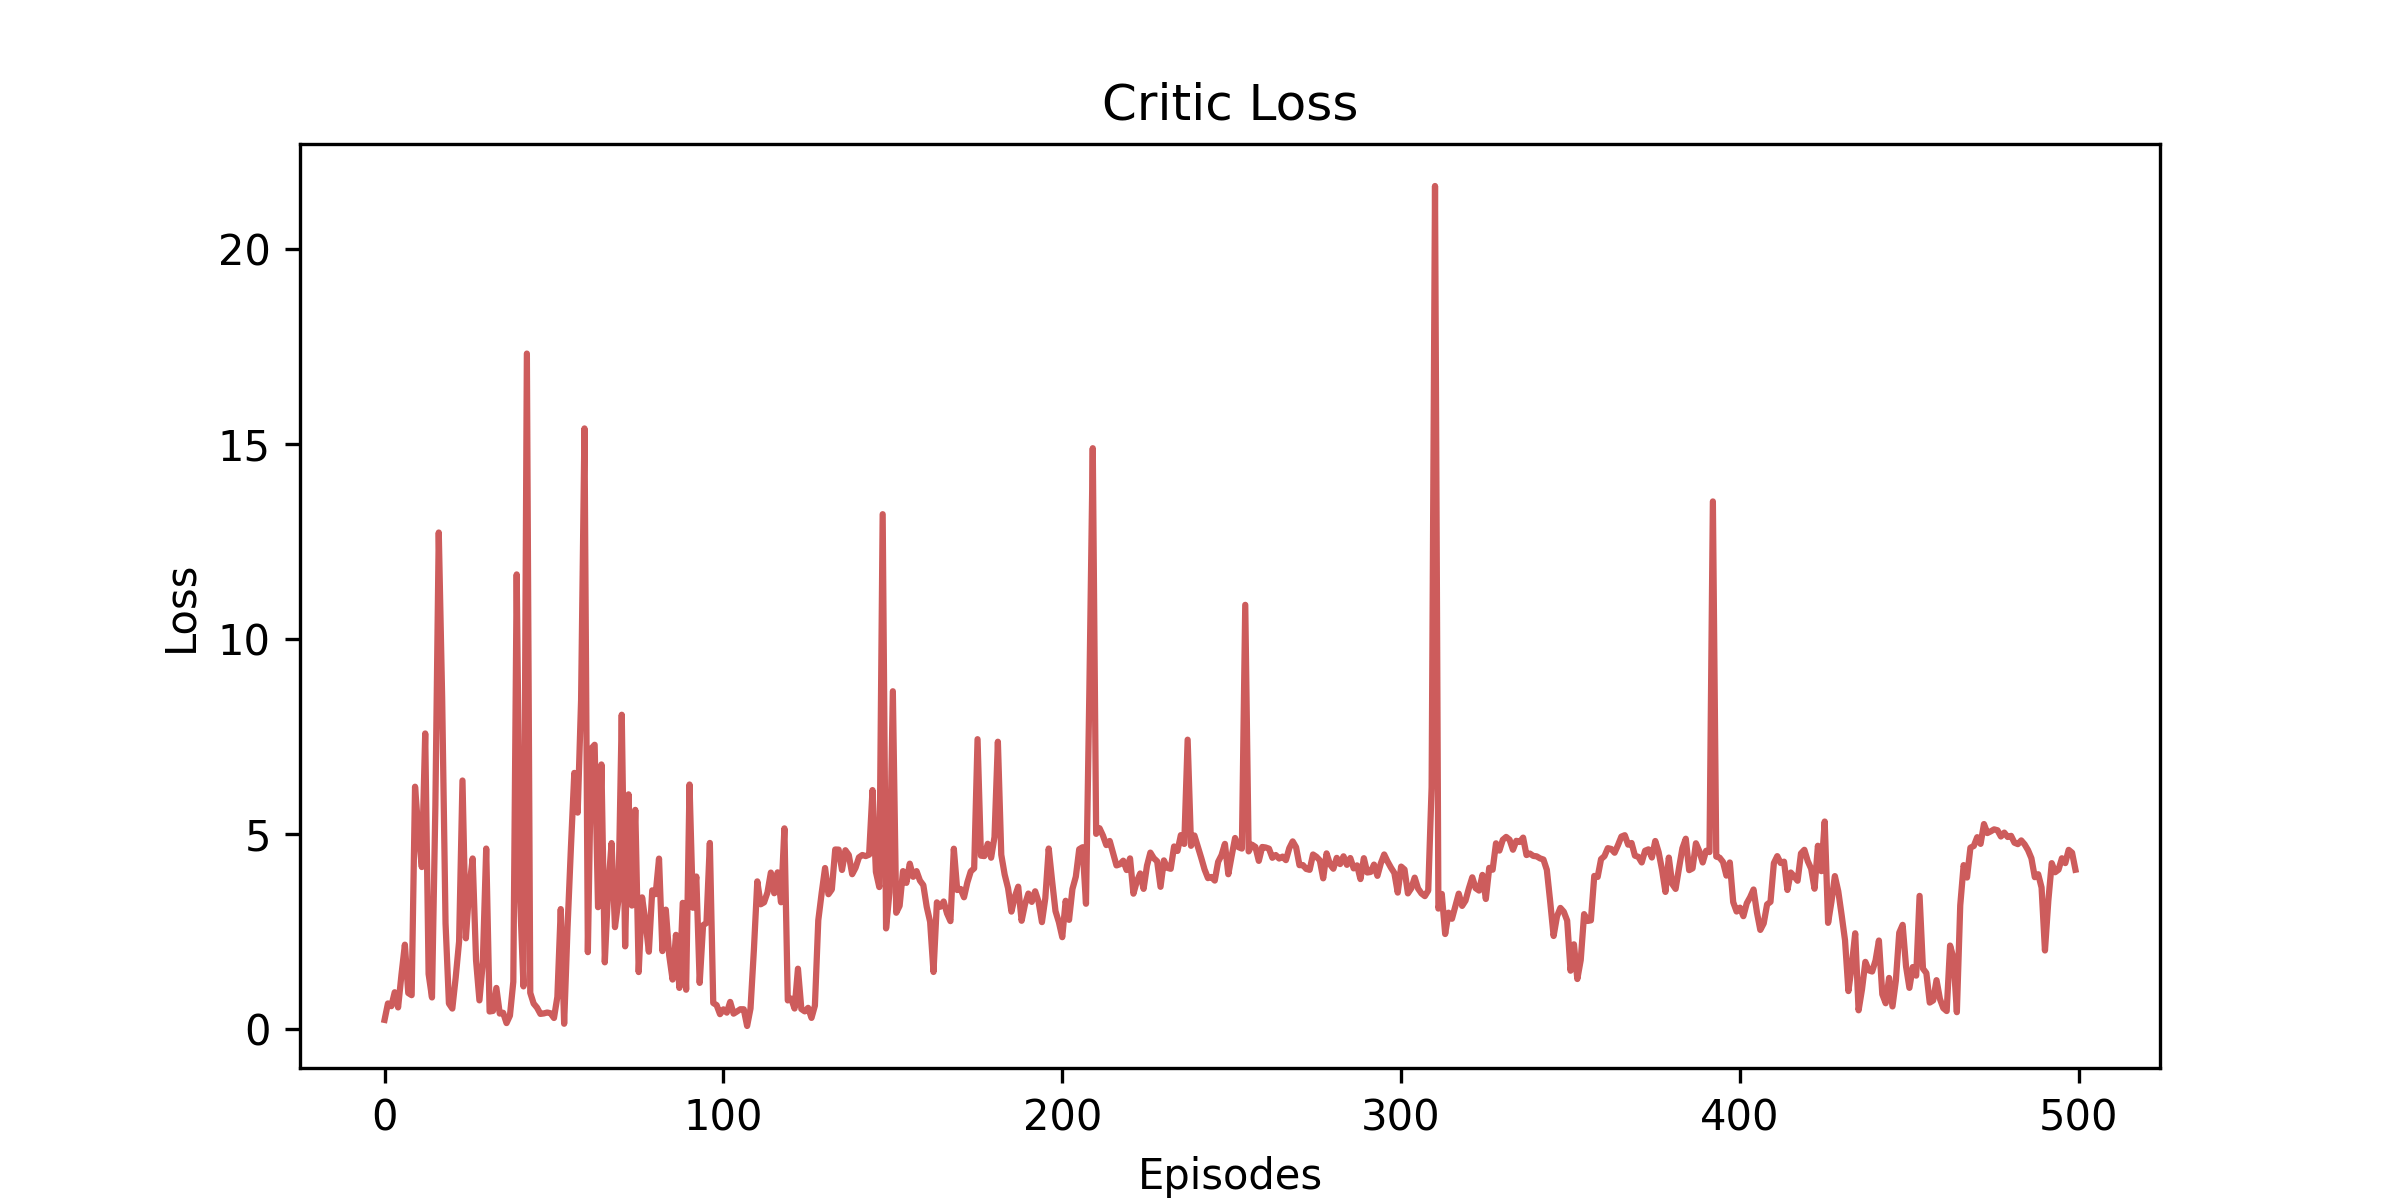
\includegraphics[width=0.8\textwidth]{../Figure/ppo_cartpole_critic_loss.png} 
        \caption{训练过程中Critic损失值的变化}
        \label{fig:critic_losses}
    \end{figure}

    图\ref{fig:ratios}展示了训练过程中概率比率的变化情况。可以看到，随着训练的进行，ratio值在1左右叫小范围波动，这表明新策略与旧策略之间的差异在逐渐减小。同时也可以注意到受算法中Clip截断以及自适应KL惩罚的影响，ratio值并未出现过大的偏离，这验证了这些方法子啊限制策略更新幅度方面的有效性。

    \begin{figure}[htbp]
        \centering
        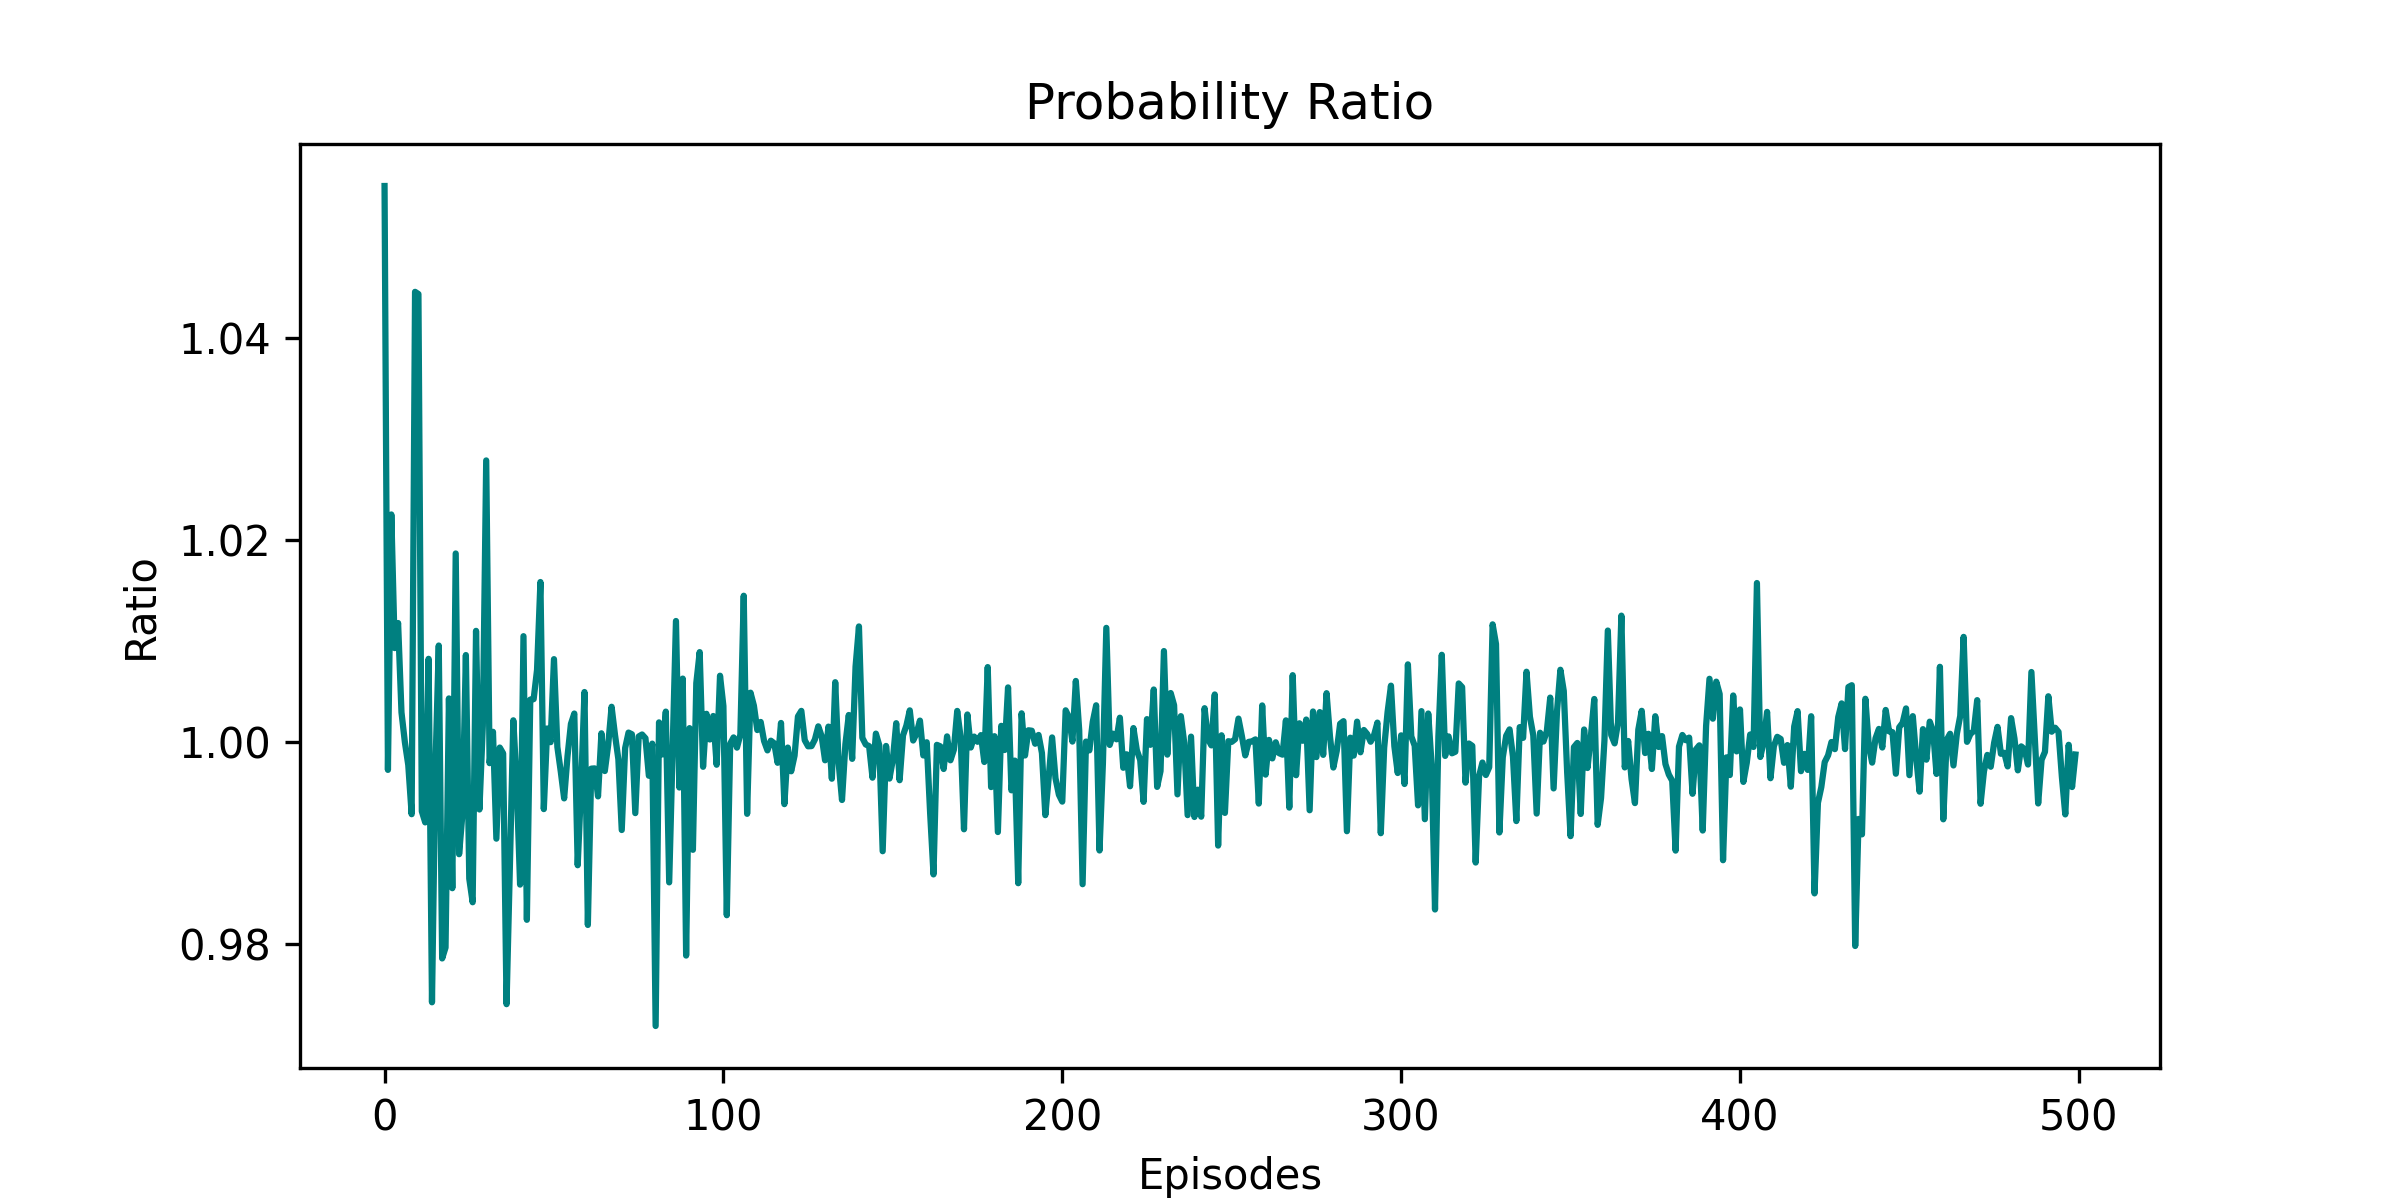
\includegraphics[width=0.8\textwidth]{../Figure/ppo_cartpole_ratio.png} 
        \caption{训练过程中ratio的变化}
        \label{fig:ratios}
    \end{figure}

    \subsection{模型演示情况}

    经过500个episode的训练，在实际演示过程中，模型在共计5次尝试中均成功将倒立摆保持在平衡状态达到了最大步数500步。
    \begin{figure}[htbp]
        \centering
        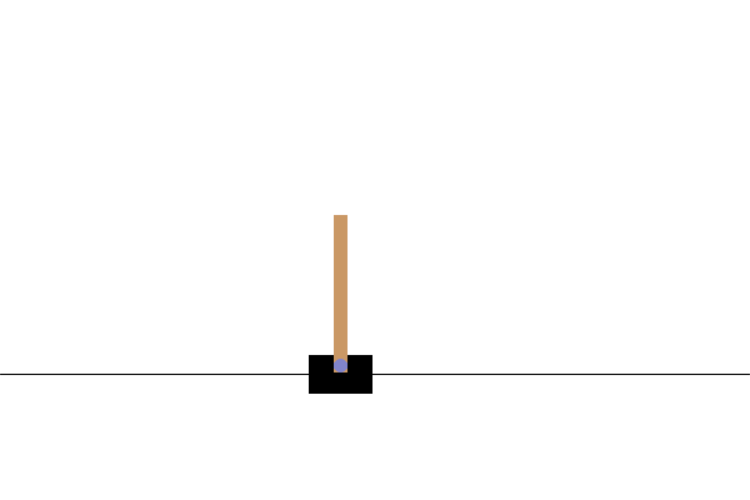
\includegraphics[width=0.8\textwidth]{../Figure/Show.png} 
        \caption{实际运行情况}
        \label{fig:show}
    \end{figure}

	\section{总结}
    本次作业中，成功实现了PPO算法并应用于倒立摆控制任务。通过Clip截断机制和自适应KL惩罚，有效提升了训练的稳定性和策略的性能。最终的模型能够稳定实现倒立摆500步的控制目标。
    
\end{document}
